\documentclass[12pt,a4paper]{article}
\usepackage[utf8]{inputenc}
\usepackage[spanish]{babel}
\usepackage{amsmath}
\usepackage{amsfonts}
\usepackage{amssymb}
\usepackage[left=2cm,right=2cm,top=2cm,bottom=2cm]{geometry}
\usepackage[T1]{fontenc}
\usepackage{titlesec}
\usepackage{hyperref}
\hypersetup{
    colorlinks=true,
    linkcolor=blue,
    urlcolor=red,
    pdftitle={Tarea 5 Viajero búsqueda local},
    }
\author{Lic. Arnoldo Del Toro Peña}
\title{Tarea 5: Algoritmo Viajero \\ Búsqueda local \\ \tiny{Algoritmo constructivo}}
\date{\today}
\usepackage{natbib}
\bibliographystyle{dinat}
\usepackage{graphicx}
\titleformat{\section}[display]
{\normalfont}{\filcenter\small
\ SECCIÓN \thesection   }
{0.5pt}{\Large\bfseries\filcenter  \hrulefill \\ }

%% %--
%\usepackage{titlesec}
%\titleformat{\section}[frame]{\normalfont} %
%{\filright\footnotesize\enspace SECCIÓN \thesection\enspace} %
%{8pt}{\Large\bfseries\filcenter} %
%%-




\begin{document}

\maketitle



\thispagestyle{empty}
\begin{abstract}
    Uso de un método metahurístico constructivo con una implementación de búsqueda local para la solución a un problema del viajero utilizando programación en python.
\end{abstract}
{\centering \textit{Palabras clave: python,viajero, metahurística, búsqueda,local.}}
\section{Introducción}
En este documento se presentarán los resultados a las instancias obtenidas, se compararán con los resultados óptimos que se presentan a continuación:
\begin{table}[h!]
\centering
\begin{tabular}{|c|c|c|c|c|}
\hline
\multicolumn{1}{|l|}{\textbf{Instancias de Prueba}} & \multicolumn{1}{l|}{\textit{Nombre de la instancia}}  & \multicolumn{1}{c|}{\textit{nodos}} & \textit{Óptimo} \\ \hline
\textit{76}                                          &  pr76.tsp                                & 76                            & 108159            \\ \hline
\textit{105}                                          & lin105.tsp                                 & 105                            & 14379             \\ \hline
\textit{280}                                          & a280.tsp                                 & 280                           &2579            \\ \hline
\textit{130}                                          & ch130.tsp                                 & 130                            & 6110             \\ \hline
\textit{225}                                          & tsp225.tsp                                 & 225                            & 3919             \\ \hline

\end{tabular}
\end{table}

Más adelante analizaremos las diferencias entre estos resultados y los que obtuvimos.

\section{Descripción}
 El algoritmo que se utilizó fue un algoritmo constructivo con la fórmula visto en clase, el valor de $\alpha$ se tomó de forma aleatoria al igual el nodo de inicio, se corrieron 5 veces cada instancia como se pedía.
 
 Los resultados se presentan en el repositorio de git hub, en el archivo con nombre resultados.txt, más adelante se presentarán en el apartado de resultados.
 
 El algoritmo se basa en la selección de las mejores opciones, que se seleccionan en base a los valores obtenidos de la fórmula.

 Posteriormente a esto se implementó una búsqueda local, en el cual se intercambiaron dos nodos, se almacenó en una variable delta y se comparó con el valor antes del intercambio, si este mejoraba la solución se mantenía el cambio, de otro modo no se hacía el cambio, en el código
 se imprime un mensaje si se realiza este mismo, al final el código imprime el mejor valor objetivo obtenido y su respectiva ruta junto con el valor antes de la búsqueda local.
 
 \section{Descripción del algoritmo constructivo}

 Como se mencionó anteriormente, la selección del nodo siguiente se baso en una lista generada por los nodos que estaban entre un cierto rango el cual esta determinado por la siguiente fórmula:

 \[ c_{min} \leq c_e \leq c_{min} + \alpha * (c_{max} - c_{min}) \]
\newline
 Donde $c_e$ es el costo de los nodos disponibles para visitar, una vez generada la lista seleccionamos al azar un nodo de esta misma, el cual será el nodo próximo a visitar.

 Esto lo repetimos hasta que todos los nodos esten visitados, agregando el nodo inicial para terminar el recorrido del agente viajero.

\section{Descripción del algoritmo búsqueda local}
 El algoritmo se finaliza cuando todos los nodos estan marcados y tenemos que agregar el nodo inicial al final para poder cerrar el recorrido.Podemos enumerar sus pasos de la siguiente manera:
\begin{enumerate}
    \item Elección de un vértice arbitrario respecto al vértice actual.
    \item Descubra la arista de menor distancia que ya este conectada al vértice actual y a un vértice no visitado V.
    \item Convierta el vértice actual en V.
    \item Marque V como visitado.
    \item Si todos los vértices del dominio estuvieran visitados, cierre el algoritmo.
    \item Vaya al paso 2
\end{enumerate}
El algoritmo de búsqueda local sigue los siguientes pasos:
\begin{enumerate}
    \item Seleccionamos los nodos a intercambiar.
    \item Si los nodos son adyacentes entonces: calculamos el delta de la siguiente manera $$C_{act} = C_{i-1,i}+C_{i,j}+C_{j,j+1}$$, $$C_{nue} = C_{i-1,j}+C_{j,i}+C_{i,j+1}$$ $$\delta = C_{act} - C_{nue}$$
    \item Si no, calculamos el delta de la siguiente manera: $$C_{act} = C_{i-1,i}+C_{i,i+1}+C_{j-1,j}+C_{j,j+1}$$, $$C_{nue} = C_{i-1,j}+C_{j,i+1}+C_{j-1,i}+C_{i,j+1}$$ $$\delta = C_{act} - C_{nue}$$
    \item Si $\delta \geq 0$ entonces intercambiamos los nodos.
    \item Si no hemos hecho esto para todos los nodos regresamos al paso 1. 
\end{enumerate}
\section{Implementación} 
El algoritmo se programó en lenguaje python con referencias en \cite{van1991guia}, \cite{van2017tutorial} y \cite{chun2001core}, y se puede verificar en el siguiente repositorio de: \href{https://github.com/arnoldae9/PycharmProjects.git}{git-hub}.

\section{Resultados} 
Los resultados se pueden ver en el mismo enlace de git-hub, en los documentos txt, sin embargo se presentarán a continuación en una forma más ordenada:
\\ En el archivo de resultados.txt podemos encontrar todos los resultados obtenidos de cada una de las 5 iteraciones en cada instancia. 
\begin{table}[h!]
    \centering
    \resizebox*{15 cm}{!}{\begin{tabular}{|c|c|c|c|c|c|c|}
        \hline
        \multicolumn{1}{|l|}{\textbf{Instancias de Prueba}} & \multicolumn{1}{l|}{\textit{Nombre de la instancia}}  & \multicolumn{1}{c|}{\textit{nodos}} & \textit{Óptimo} & \textit{Mejor valor} &\textit{promedio}         \\ \hline
        \textit{76}                                          &  pr76.tsp                                & 76                            & 108159                            &166453.37            &171376.45        \\ \hline
        \textit{105}                                          & lin105.tsp                                 & 105                            & 14379                         &36453.17             &37152.48         \\ \hline
        \textit{130}                                          & ch130.tsp                                 & 130                            & 6110                           &47585.29             &47996.23    \\ \hline
        \textit{225}                                          & tsp225.tsp                                 & 225                            & 3919                          &9897.72              &10278.02    \\ \hline
        \textit{280}                                          & a280.tsp                                 & 280                           & 2579                             &3447.23              &3845.32            \\ \hline
        \end{tabular}}
    \end{table}

A continuación se muestran las gráficas de los valores de las funciones objetivo obtenidas:
\begin{figure}[h!t]
    \begin{minipage}[b]{0.4\linewidth}
    \centering
    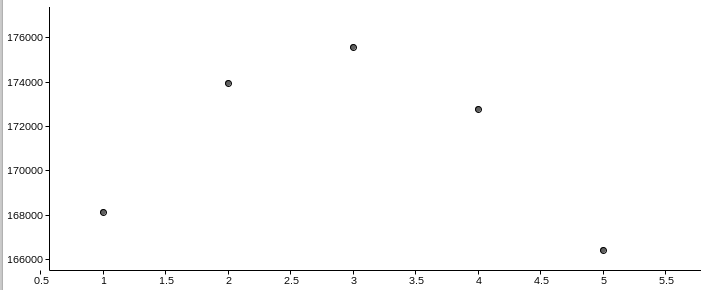
\includegraphics[scale = 0.2]{pr76.png}
    \caption{pr 76}
    \end{minipage}
    \hspace{0.5cm}
    \begin{minipage}[b]{0.4\linewidth}
    \centering
    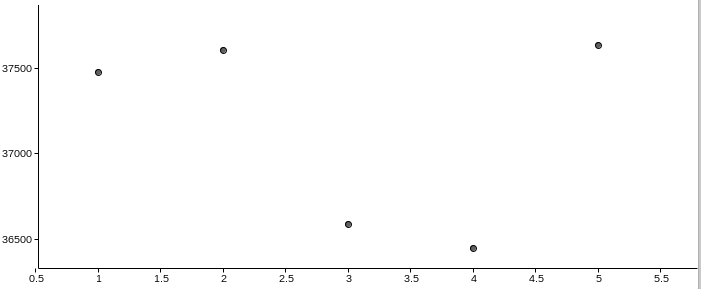
\includegraphics[scale = 0.2]{lin105.png}
    \caption{lin 105}
    \end{minipage}
\end{figure}

\begin{figure}[h!t]
    \begin{minipage}[b]{0.4\linewidth}
    \centering
    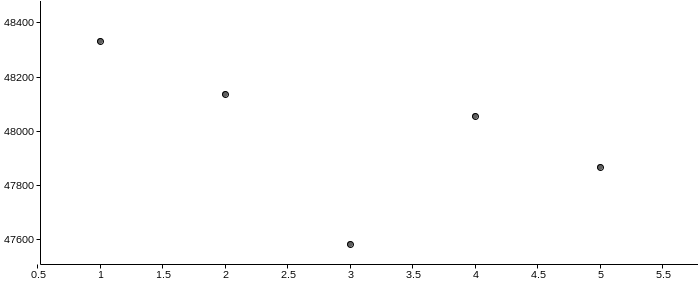
\includegraphics[scale = 0.2]{ch130.png}
    \caption{ch130}
    \end{minipage}
    \hspace{0.5cm}
    \begin{minipage}[b]{0.4\linewidth}
    \centering
    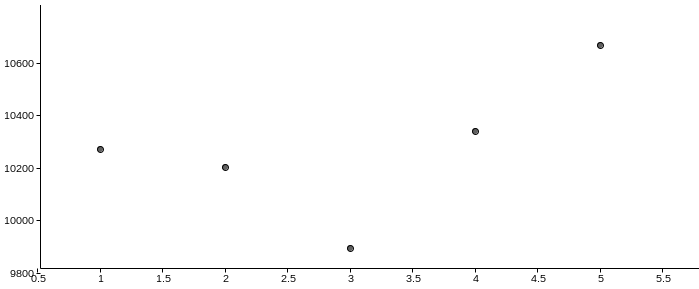
\includegraphics[scale = 0.2]{tsp225.png}
    \caption{tsp225}
    \end{minipage}
\end{figure}

\begin{figure}[h!t]
\centering
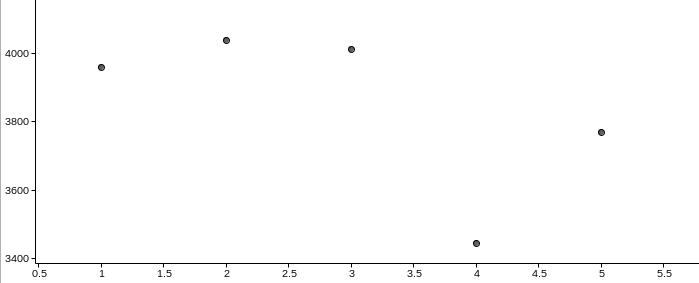
\includegraphics[scale = 0.2]{a280.png}
\caption{a280}
\end{figure}

\newpage
Como podemos ver todos los valores se representan de manera totalmente dispersa, esto se debe a que en algunos casos el valor de alfa es muy alto.

En una segunda ejecución del algoritmo se fijo alfa a 0.1 y se obtuvieron mejores resultados, estos mismos se pueden encontrar en el archivo resultadosalfa0\_1.txt en el mismo repositorio.

\section{Mejoras}

Se comprobó lo que ya sabiamos, al tomar alfa muy alto prácticamente las soluciones son aleatorias, sin tomar las mejoras opciones para el siguiente nodo.
\newline Se mejoró la solución con un algoritmo de búsqueda local, utilizando el mismo nodo y la solución obtenida del algoritmo anterior.
\section{Conclusiones} 
No es conveniente dejar aleatorio el valor de alfa, ya que se obtienen resultados muy lejos de la respuesta sin importar la ejecución de la búsqueda local.
\newpage
\bibliography{biblio}
\end{document}
